\section*{Условие}
Используя хвостовую рекурсию, разработать программу, позволяющую найти:
\begin{enumerate}
	\item n!;
 	\item n-e число Фибоначчи.
\end{enumerate}
Для каждой программы реализовать два варианта: с использованием отсечения и без использования отсечения.  

Убедиться в правильности результатов.

\textbf{Для одного} из вариантов \textbf{ВОПРОСА} и каждого задания \textbf{составить
таблицу}, отражающую конкретный порядок работы системы:

Т.к. резольвента хранится в виде стека, то состояние резольвенты требуется отображать
в столбик: (вершина – сверху). Новый шаг надо начинать с нового состояния резольвенты.  

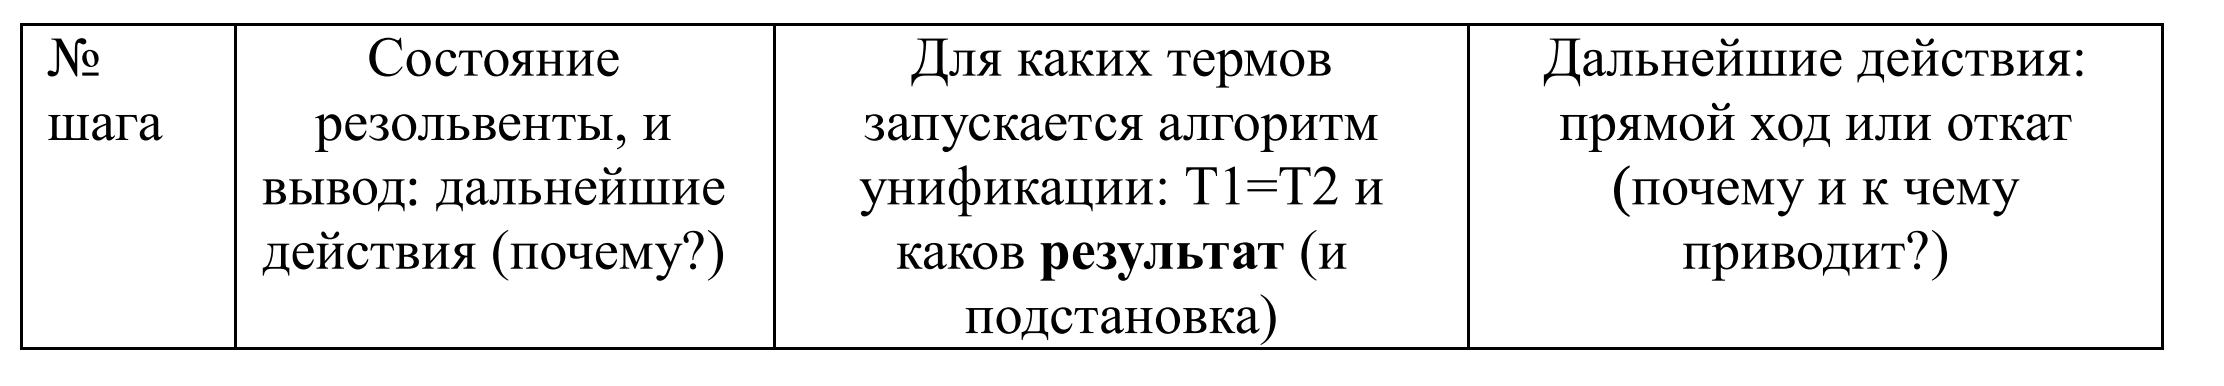
\includegraphics[scale=0.4]{./inc/img/tb_tmpl}

\section*{Решение}
\lstinputlisting[caption={Факториал}, label={lst:t1}, language=Prolog]{../src/fact_tail.pro}

В Таблице \ref{tbl:1} представлен порядок поиска ответа на вопрос 1.

\begin{landscape}
    \setlength{\LTcapwidth}{\linewidth}
    \begin{longtable}{|c|c|c|c|c|}
        \caption[Порядок формирования результата для 1-го вопроса]{Порядок формирования результата для 1-го вопроса} \label{tbl:1}\\
    
        \hline
            Шаг & Сравниваемые термы; & Дальнейшие & Резольвента & Подстановка \\
                & результаты & действия & & \\
        \endfirsthead
    
        \multicolumn{5}{l}
        {{\tablename\ \thetable{} -- продолжение}} \\
        \hline 
            Шаг & Сравниваемые термы; & Дальнейшие & Резольвента & Подстановка \\
                & результаты & действия & & \\\hline
        \endhead
        
        \hline \multicolumn{5}{|r|}{{Продолжение на следующей странице}} \\ \hline
        \endfoot
        
        \hline \multicolumn{5}{|r|}{{Конец таблицы}} \\ \hline
        \endlastfoot
        
        \hline
              & fib(9, R) & Прямой ход & fib(9, R) & \\
            1 & и fib(0, 0) & Переход к & &\\
			  & Не унифицируемы & след. предл. & &\\
			\hline
			\dots & \dots & \dots & \dots & \dots \\
			\hline 
			3 & fib(9, R) & Прямой ход & fib(9, 0, 1, Result) & N = 9\\
              & и fib(N, Result) & & &\\
            \hline
			\dots & \dots & \dots & \dots & \dots \\
		    \hline 
			  & fib(9, 0, 1, Result) & Прямой ход & 9 > 0 & N = 9\\
            8 & и fib(N, Prev1, Prev2, Result) & & New\_Prev2 = 0 + 1 & Prev1 = 0\\
              & & & N1 = 9 - 1 & Prev2 = 1\\
              & & & fib(N1, 1, New\_Prev2, Result) &\\
            \hline 
			  & & Прямой ход & New\_Prev2 = 0 + 1 & N = 9\\
            9 & 9 > 0 & & N1 = 9 - 1 & Prev1 = 0\\
              & & & fib(N1, 1, New\_Prev2, Result) & Prev2 = 1\\
            \hline 
			10 & New\_Prev2 is 0 + 1 & Прямой ход & N1 is N - 1 & N = 9\\
              & & & fib(N1, 1, 1, Result) & Prev1 = 0\\
              & & & & Prev2 = 1\\
              & & & & New\_Prev2 = 1\\
            \hline 
			11 & N1 = 8 - 1 & Прямой ход & fib(8, 1, 1, Result) & N = 9\\
              & & & & Prev1 = 0\\
              & & & & Prev2 = 1\\
              & & & & N1 = 8\\
            \hline
			\dots & \dots & \dots & \dots & \dots \\
            \hline 
			16 & fib(8, 1, 1, Result) & Прямой ход & 8 > 0 & N = 8\\
              & и fib(N, Prev1, Prev2, Result) & & New\_Prev2 is 1 + 1 & Prev1 = 1\\
              & & & N1 = 8 - 1 & Prev2 = 1\\
              & & & fib(N1, 1, New\_Prev2, Result) & \\
            \hline 
			63 & fib(0, 34, 55, Result) & Прямой ход & ! & N = 34\\
              & и fib(0, N, \_, N) & & & \\
			\hline
            64  & ! & Завершение & & R = 34 \\
              & & работы & &\\
              & & 1 подст. & & \\
              & & в рез-те & & \\
    \end{longtable}
\end{landscape}

\lstinputlisting[caption={Фибоначчи}, label={lst:t2}, language=Prolog]{../src/fib_tail.pro}

В Таблице \ref{tbl:2} представлен порядок поиска ответа на вопрос 1.

\begin{landscape}
    \setlength{\LTcapwidth}{\linewidth}
    \begin{longtable}{|c|c|c|c|c|}
        \caption[Порядок формирования результата для 1-го вопроса]{Порядок формирования результата для 1-го вопроса} \label{tbl:2}\\
    
        \hline
            Шаг & Сравниваемые термы; & Дальнейшие & Резольвента & Подстановка \\
                & результаты & действия & & \\
        \endfirsthead
    
        \multicolumn{5}{l}
        {{\tablename\ \thetable{} -- продолжение}} \\
        \hline 
            Шаг & Сравниваемые термы; & Дальнейшие & Резольвента & Подстановка \\
                & результаты & действия & & \\\hline
        \endhead
        
        \hline \multicolumn{5}{|r|}{{Продолжение на следующей странице}} \\ \hline
        \endfoot
        
        \hline \multicolumn{5}{|r|}{{Конец таблицы}} \\ \hline
        \endlastfoot
        
        \hline
              & fact(9, R) & Прямой ход & fact(9, R) & \\
            1 & и fact(0, 0, Result) & Переход к & &\\
			  & Не унифицируемы & след. предл. & &\\
			\hline
			\dots & \dots & \dots & \dots & \dots \\
			\hline 
			3 & fact(9, R) & Прямой ход & fact(9, 1, Result) & N = 9\\
              & и fact(N, R) & & &\\
            \hline
			\dots & \dots & \dots & \dots & \dots \\
		    \hline 
			  & fact(9, 1, Result) & Прямой ход & NewN = 9 - 1 & N = 9\\
            5 & и fact(N, Acc, Result) & & NewAcc = 1 * 9 & Acc = 1\\
              & & & fact(NewN, NewAcc, Result) & \\
            \hline 
			6 & NewN = 9 - 1 & Прямой ход & NewAcc = 1 * 9 & N = 9\\
              & & & fact(8, NewAcc, Result) & Acc = 1\\
              & & & & NewN = 8\\
            \hline 
			7 & NewAcc = 1 * 9 & Прямой ход & fact(8, 9, Result) & N = 9\\
              & & & & Acc = 1\\
              & & & & NewN = 9\\
              & & & & NewAcc = 9\\
            \hline
			\dots & \dots & \dots & \dots & \dots \\
            \hline 
			0 & fact(0, 362880, Result) & Прямой ход & ! & N = 0\\
               & fact(0, Result, Result) & & & R = 362880\\
			\hline
            0 & ! & Завершение & & R = 362880 \\
              & & работы & &\\
              & & 1 подст. & & \\
              & & в рез-те & & \\
    \end{longtable}
\end{landscape}

\section*{Контрольные вопросы}

\subsection*{Что такое рекурсия?}

Рекурсия – это способ заставить систему
использовать многократно одну и ту же процедуру.

\subsection*{Как организуется хвостовая рекурсия в Prolog?}

\begin{itemize}
    \item рекурсивный вызов один, расположен в конце тела правила;
    \item не должно быть возможности сделать откат до вычисления рекурсивного вызова.
\end{itemize}

\subsection*{Как организовать выход из рекурсии в Prolog?}

С помощью отсечения

\subsection*{Какое первое состояние резольвенты?}

Заданный вопрос (goal).

\subsection*{В каком случае система запускает алгоритм унификации?}

Система запускает алгоритм унификации автоматически при необходимости доказать что-то.

\subsection*{Каково назначение и результат использования алгоритма унификации?}

Унификация – логический вывод. Результат – подстановка.

\subsection*{В каких пределах программы переменные уникальны?}

Именованная переменная уникальна в предложении, в котором она используется. Анонимные переменные всегда уникальны.

\subsection*{Как применяется подстановка, полученная с помощью алгоритма унификации?}

Подстановка применяется к целям в резольвенте путем замены текущей переменной на соответствующий терм.

\subsection*{Как изменяется резольвента?}

Преобразования резольвенты выполняются с помощью редукции. Редукцией цели G с помощью программы P называется замена цели G телом того правила из P, заголовок которого унифицируется с целью. Новая резольвента образуется в два этапа:
\begin{itemize}
    \item в текущей резольвенте выбирается одна из подцелей и для неё выполняется редукция;
    \item к полученной конъюнкции целей применяется подстановка, полученная как наибольший общий унификатор цели и заголовка сопоставленного с ней правила.
\end{itemize}

\subsection*{В каких случаях запускается механизм отката?}

Механизм отката запустится в случае неудачи алгоритма унификации.